\chapter{Методика и средства компонентного проектирования интерфейсов ostis-систем}
\chapauthortoc{Садовский М.~Е.\\Жмырко А.~В.}
\label{chapter_ui_design}

\vspace{-7\baselineskip}

\begin{SCn}
\begin{scnrelfromlist}{автор}
	\scnitem{Садовский М.~Е.}
	\scnitem{Жмырко А.~В.}
\end{scnrelfromlist}
\bigskip
	
\begin{scnrelfromlist}{подраздел}
	\scnitem{\ref{sec_analysis_UI_design_methodologies}~\nameref{sec_analysis_UI_design_methodologies}}
	\scnitem{\ref{sec_reusable_UI_components}~\nameref{sec_reusable_UI_components}}
\end{scnrelfromlist}	
	
	
\scntext{аннотация}{Проектирование интерфейса – это один из наиболее важных  этапов разработки любой системы.
Пользователь при обращении с интерфейсом должен представить себе, какая информация о выполняемой задаче у него существует, и в каком состоянии находятся средства, с помощью которых он будет решать данную задачу. Эффективность работы пользователя и его интерес обеспечивает правильно сформулированная \myuline{методика разработки и проектирования пользовательского интерфейса}. \newline
В настоящее время организация взаимодействия пользователя с компьютерной системой основана на парадигме \myuline{грамотного пользователя}, который знает, как управлять системой и несёт полную ответственность за качество взаимодействия с ней.
Многообразие форм и видов интерфейсов приводит к необходимости пользователя  адаптироваться к каждой конкретной системе, обучаться принципам взаимодействия с ней для решения необходимых ему задач. \newline
Проектирование \textit{пользовательских интерфейсов} включает в себя ряд последовательных этапов.
В рамках главы рассмотрены этапы проектирования \textit{пользовательских интерфейсов} и этапы проектирования \textit{адаптивных интеллектуальных мультимодальных пользовательских интерфейсов}.}
\end{SCn}

\section{Анализ методик проектирования пользовательских интерфейсов}
\label{sec_analysis_UI_design_methodologies}

\begin{SCn}
	\begin{scnrelfromlist}{подраздел}
		\scnitem{\ref{sec_UI_analisys}~\nameref{sec_UI_analisys}}
	\end{scnrelfromlist}
\end{SCn}

Методика проектирования \textit{пользовательских интерфейсов} является важной частью Технологии OSTIS, так как она описывает сам процесс проектирования.

Среди существующих методик проектирования \textit{адаптивных интеллектуальных мультимодальных пользовательских интерфейсов} можно выделить методики,
предложенные в \scncite{Ehlert2003} и  \scncite{Kong2011}.

В рамках работы \scncite{Ehlert2003} выделяется 4 основных этапа проектирования:
\begin{textitemize}
    \item анализ;
    \item разработка интерфейса;
    \item оценка интерфейса;
    \item доработка и усовершенствование.
\end{textitemize}

Этап анализа является, вероятно, самой важной фазой в любом процессе проектирования, но тем более в проектировании \textit{интерфейсов ostis-систем}. В
процессе проектирования традиционного интерфейса
необходимо проанализировать, кто является обычным пользователем, какие задачи \textit{интерфейс} должен поддерживать. 

В \textit{пользовательском интерфейсе} часто нет среднего пользователя.
В идеале, \textit{пользовательский интерфейс} должен быть способен адаптироваться к любому пользователю в любой среде. Поэтому используемая техника адаптации должна быть разработана таким образом, чтобы она могла поддерживать все типы пользователей.

Этап \textit{анализа} включает выполнение четырех взаимосвязанных видов анализа:
\begin{textitemize}
    \item \textit{функциональный анализ};
    \item \textit{анализ данных};
    \item \textit{анализ пользователей};
    \item \textit{анализ среды}.
\end{textitemize}

В рамках \textit{функционального анализа} необходимо дать ответ на вопрос: "каковы \uline{основные функции системы}?".
В рамках \textit{анализа данных} необходимо определить \uline{значение и структуру данных}, используемых в приложении.
В рамках \textit{анализа пользователей} необходимо выделить \uline{типы пользователей и их возможности} в интеллектуальном
и когнитивном плане.
В рамках \textit{анализа среды} необходимо определить \uline{требования, предъявляемые к среде}, в которой будет работать система.

Результатом данного этапа является \uline{cпецификация целей и информационных потребностей пользователя}, а также
\uline{спецификация функций и информации}, которые требуются системе.
\textit{Разработка интерфейса} включает следующие шаги:
\begin{textitemize}
	\item \textit{создание модели интерфейса} в соответствии с этапом анализа;
	\item реализация модели интерфейса.
\end{textitemize}

Результатом данного этапа является \textit{пользовательский интерфейс}, который, по мнению разработчика, удовлетворяет требованиям пользователей и соответствует требованиям, сформулированным на этапе анализа.

\textit{Оценка интерфейса} предполагает, что:
\begin{textitemize}
	\item требования, которые были сформулированы на этапе \textit{анализа}, должны быть удовлетворены;
	\item эффективность модели интерфейса должна быть исследована.
\end{textitemize}

На этапе \textit{оценки интерфейса} необходимо вернуться к требованиям \textit{этапа анализа}. Требования, которые
были сформулированы на \textit{этапе анализа}, должны быть выполнены, а также должна быть исследована эффективность модели интерфейса.
Чтобы определить эту эффективность, необходимо определить критерии эффективности.

Очень важным, но субъективным критерием является удовлетворенность пользователя. Поскольку пользователь должен работать с \textit{интерфейсом}, он имеет право голоса в вопросе о том, удобно ли работать с \textit{интерфейсом} и т.п.

Критериями эффективности могут выступать различные показатели, такие как:
\begin{textitemize}
	\item количество ошибок;
	\item время выполнения задачи;
	\item отношение пользователя к интерфейсу;
	\item и так далее.
\end{textitemize}

\textit{Доработка и усовершенствование} осуществляется на основе проблем, выявленных на этапе оценки. В рамках данного этапа вносится ряд улучшений в модель \textit{интерфейса}. Затем начинается новый цикл проектирования. Этот итеративный процесс будет продолжаться до тех пор, пока результат оценки не будет удовлетворять обозначенным требованиям. 

Методика, предложенная в \scncite{Kong2011} включает 6 этапов:
\begin{textitemize}
	\item моделирование пользовательского интерфейса (описание абстрактного пользовательского интерфейса);
	\item проектирование пользовательского интерфейса по умолчанию (стандартная версия, конкретный пользовательский интерфейс);
	\item разработка пользовательского интерфейса (расширение или замена пользовательского интерфейса по умолчанию) - этот шаг опускается, когда система генерирует пользовательский интерфейс по умолчанию автоматически;
	\item создание контекста использования (идентификация и создание контекста использования - модели пользователя, модель устройства и модель среды/платформы);
	\item адаптация пользовательского интерфейса - автоматически - (адаптация пользовательского интерфейса во время выполнения для соответствия конкретного контекста использования);
	\item кастомизация пользовательского интерфейса - настройка пользовательского интерфейса самим пользователем (адаптируемость).
\end{textitemize}

На основе рассмотренных методик проектирования интерфейсов можно выделить следующие общие этапы:
\begin{textitemize}
\item \textit{анализ контекста использования и задач пользователей};
\item \textit{проектирование и разработка интерфейса};
\item \textit{оценка качества спроектированного интерфейса}.
\end{textitemize}

Среди недостатков предложенных подходов можно выделить:
\begin{textitemize}
	\item знания по каждому этапу проектирования находятся у разных специалистов в неформализорованном неунифицированном виде;
	\item отсутствие \textit{этапа формализованного документирования} этапов проектирования приводит в дальнейшем к необходимости создания отдельных help-систем для пользователей, разработчиков и так далее.
\end{textitemize}

На основе проведенного анализа предлагается использовать онтологический подход на основе семантической модели в процессе проектирования и реализации \textit{адаптивного интеллектуального мультимодального пользовательского интерфейса}. Такой \textit{интерфейс} предлагается рассматривать как специ-
ализированную подсистему для решения \textit{интерфейсных задач} пользователя, состоящую из \textit{базы знаний} и \textit{решателя задач}. 

Описание модели \textit{базы знаний} и \textit{решателя задач} предлагается осуществлять на основе универсального унифицированного \textit{языка представления знаний}, что обеспечит \myuline{совместимость} между этими компонентами.

Архитектура \textit{интерфейса} такой системы была рассмотрена на рисунке \nameref{fig:archit_intel_system}.

\begin{figure}[h]
	\centering
	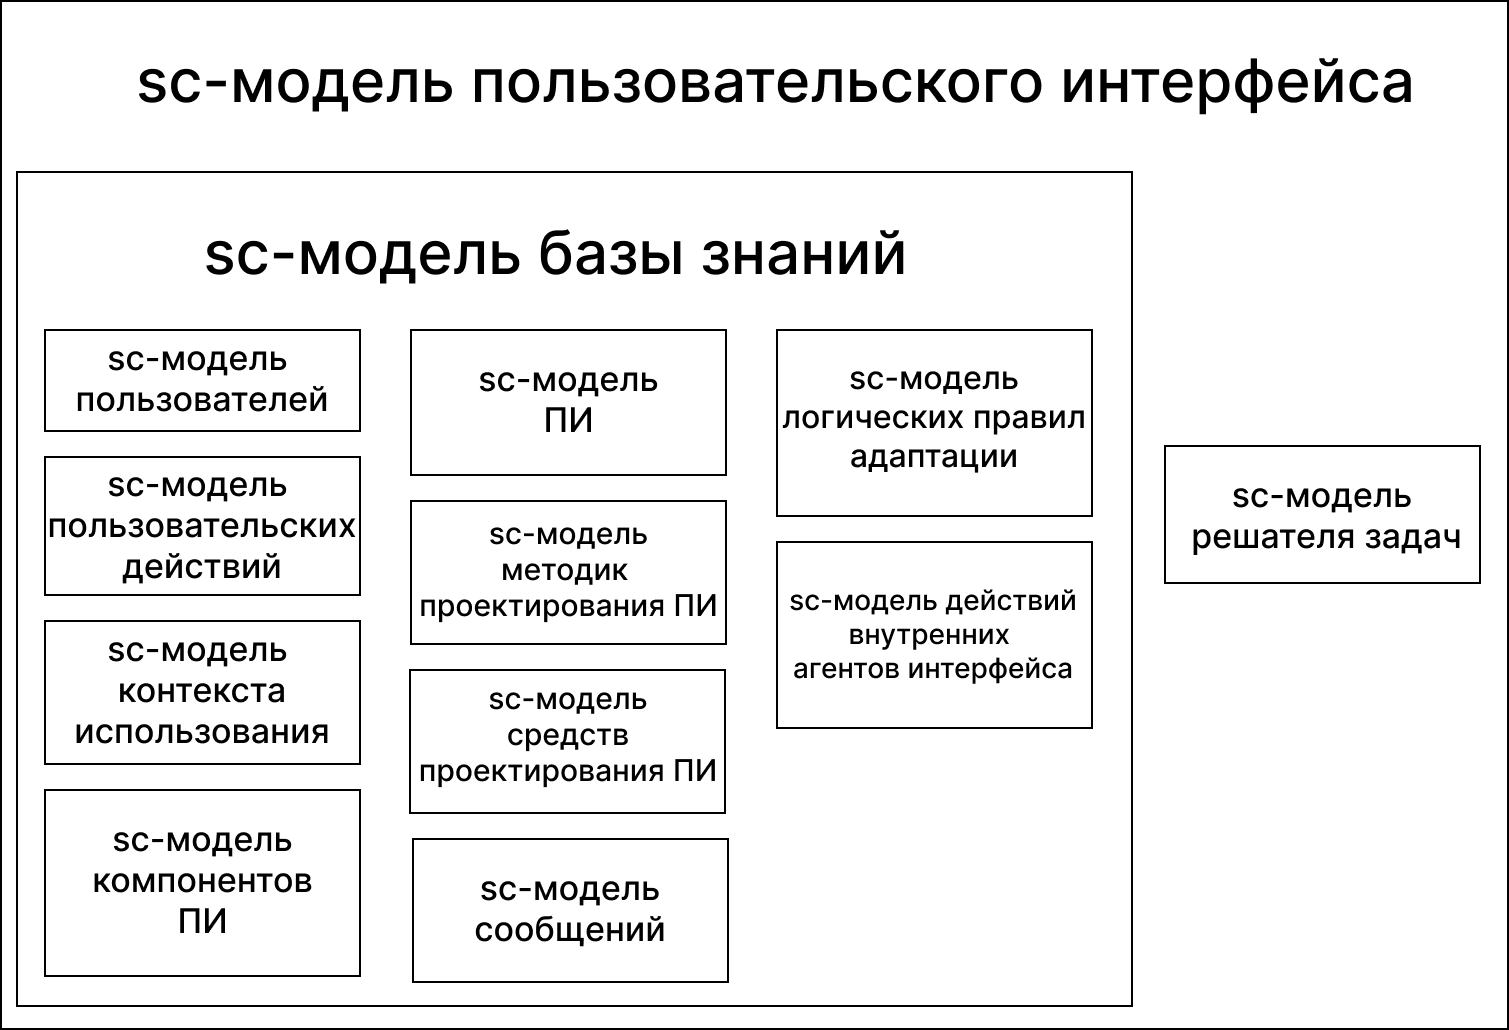
\includegraphics[scale=0.2]{images/part5/sc-model-ui.png}
	\caption{Архитектура интеллектуального интерфейса}
	\label{fig:archit_intel_system}
\end{figure}

Таким образом, предлагаемая методика проектирования \textit{интерфейсов ostis-систем} будет включать:
\begin{textitemize}
\item анализ пользователя, его задач и целей, а также контекста использования;
\item анализ требований к пользовательскому интерфейсу и спецификация проектируемого пользовательского интерфейса;
\item задачно-ориентированная декомпозиция;
\item проектирование пользовательского интерфейса по умолчанию;
\item разработка пользовательского интерфейса;
\item анализ пользовательского интерфейса и его адаптации.
\end{textitemize}

Поскольку знания о конкретном этапе обычно находятся у разных экспертов, особенностью предлагаемого подхода является обязательное формализованное документирование знаний в унифицированном виде и применение на каждом из этапов компонентного подхода.

Для применения компонентного подхода предлагается использовать \textit{библиотеку многократно используемых компонентов} базы знаний, решателя задач и интерфейса.

\textbf{Анализ пользователя, его задач и целей, а также контекста использования}

Результаты первого этапа, такие как: модель конкретного пользователя, его потребности и контекст использования системы (устройство, окружающая среда) должны быть формализованы в рамках соответствующих онтологий базы знаний интерфейса. 
При этом в процессе формализации по необходимости должны быть переиспользованы компоненты базы знаний из библиотеки многократно используемых компонентов, а новые компоненты могут пополнить эту же библиотеку.

\textbf{Анализ требований к пользовательскому интерфейсу и спецификация проектируемого пользовательского интерфейса}

Результатом второго этапа являются конечные требования к интерфейсу, которые должны быть сформулированы относительно модели пользователя и его цели, а также относительно контекста использования.

Спецификация включает в себя список задач решаемых интерфейсом, описание
внешних языков представления знаний.

Результаты должны быть также формализованы, а в процессе выполнения могут быть использованы существующие компонент базы знаний из библиотеки многократно используемых компонентов.

\textbf{Задачно-ориентированная декомпозиция}

На этапе задачно-ориентированной декомпозиции специфицированный 
интерфейс разбивается на интерфейсные подсистемы, которые могут разрабатываться
параллельно. Это позволяет сократить сроки проектирования пользовательского интерфейса.
Целесообразно проводить разбиение таким образом, чтобы максимальное количество
подсистем уже имелось в \textit{Библиотеке многократно используемых компонентов пользовательских интерфейсов ostis-систем}.

\textbf{Проектирование пользовательского интерфейса по умолчанию}

В соответствии с требованиями к пользовательскому интерфейсу, строится модель адаптивного интеллектуального мультимодального пользовательского интерфейса, которая является результатом третьего этапа.

Такая модель будет включать в себя формализованную модель базы знаний и решателя задач.

При проектировании могут быть использованы компоненты интерфейса, базы знаний и решателя задач. 
Компоненты будут записаны в унифицированном виде, что позволит обеспечить их автоматическую совместимость.

\textbf{Разработка пользовательского интерфейса}

Результатом четвертого этапа является реализация спроектированного пользовательского интерфейса. 

После разработки пользовательского интерфейса выделяются типовые
фрагменты интерфейса. Специфицируя фрагменты интерфейса необходимым образом следует включать их в библиотеку многократно используемых компонентов интерфейса.

При разработке пользовательского интерфейса также можно использовать готовые компоненты интерфейса из библиотеки многократно используемых компонентов интерфейса.



\textbf{Анализ пользовательского интерфейса и его адаптации}

На данном этапе используются готовые компоненты решателя задач.

Таким образом будет сформирована база знаний проектируемого интерфейса, которая автоматически может быть использована в качестве help-системы для пользователей, разработчиков и т.д.

\subsection{Анализ методов оценки пользовательских интерфейсов}
\label{sec_UI_analisys}

Как было сказано ранее, этап оценки пользовательских интерфейсов является достаточно важным.
Оценка пользовательского интерфейса необходима для улучшения коммуникации между интеллектуальными системами и их пользователями. Существует множество методов для оценки пользовательских интерфейсов, направленных, в основном, на выявление проблем с использованием системы и минимизацию риска ошибок. Однако до сих пор нет комплексного подхода к оценке пользовательских интерфейсов интеллектуальных систем.

При оценке пользовательских интерфейсов большую роль играет человеческий фактор, а основными участниками являются пользователи и эксперты. Очень сложно оценить правильность решения по адаптации пользовательского интерфейса интеллектуальной системы и оценить его без участия человека. Конечно, есть небольшие обобщенные правила построения пользовательских интерфейсов, такие как:

\begin{textitemize}
	\item интерфейс должен быть интуитивно понятен для конечного пользователя;
	\item интерфейс должен быть доступным для пользователей с ограниченными возможностями и пользователей, впервые сталкивающимися с информационными технологиями;
	\item достижение цели пользователем должно осуществляться наименее возможным количеством шагов.
\end{textitemize}


Оценка пользовательских интерфейсов интеллектуальных систем имеет свои особенности и требует специальных методов и инструментов.

Некоторые методы оценки пользовательских интерфейсов интеллектуальных систем включают:
\begin{textitemize}
	\item Оценку точности и полноты. 
	
	Это метод, при котором оценивается точность и полнота ответов системы на запросы пользователей.
	
	Точность означает, насколько хорошо пользовательский интерфейс отражает действительный опыт пользователя и предлагает ему наиболее подходящий контент в соответствии с его потребностями и предпочтениями. Оценить точность возможно путем анализа, насколько легко использовать интерфейс, насколько он отражает действительные возможности интеллектуальной системы и насколько он помогает пользователям достигать своих целей более эффективно.
	
	Полнота, с другой стороны, означает, насколько хорошо пользовательский интерфейс предоставляет всю необходимую информацию и функциональность, которые пользователь может потребовать в процессе взаимодействия с системой. Оценить полноту возможно путем анализа того, насколько полное и четкое описание функций, возможностей и ограничений системы предоставляется через пользовательский интерфейс, в каком объеме пользователю доступна необходимая информация для принятия решений и насколько система может эффективно реагировать на запросы и потребности пользователя.
	
	\item Оценку персонализации. 
	
	Это метод, при котором оценивается способность системы адаптироваться к потребностям и предпочтениям каждого пользователя. Оценка персонализации выполняется с помощью анализа пользовательских данных, а также проведения опросов среди пользователей, чтобы определить, насколько хорошо система учитывает их потребности.
	
	Оценка качества персонализации может включать в себя измерение следующих параметров:
	\begin{textitemize}
	\item Работоспособность - действительно ли пользовательский интерфейс адаптивный и соответствует ли он потребностям пользователя?
	\item Уникальность - насколько уникальным и индивидуальным является персонализированный пользовательский интерфейс?
	\item Понятность - насколько просто и легко пользователь может настроить и использовать персонализацию?
	\item Эффективность - насколько хорошо персонализированный пользовательский интерфейс помогает пользователю в выполнении задач?
	\item Удовлетворенность - насколько положительным и удовлетворительным является пользовательский интерфейс?
	\end{textitemize}

	Оценка персонализации адаптивных пользовательских интерфейсов может быть выполнена различными методами, включая тестирование с использованием фокус-групп, опросы пользователей, анализ данных и др.
	Важно отметить, что оценка персонализации должна проходить на всех этапах разработки для повышения пользовательского опыта и улучшения качества пользовательских интерфейсов интеллектуальных систем.
\end{textitemize}


Методы оценки пользовательских интерфейсов можно разделить на две группы: качественные и количественные.

\textbf{Качественный метод оценки пользовательских интерфейсов}
	
Задача качественных методов — помочь понять мотивы поведения, потребности и логику пользователей.
	
Качественные методы нацелены на сбор данных, описывающих предмет изучения. Они позволяют углубиться в предметную область для получения представления о мотивации, мышлении и взглядах пользователей. 
	
К качественным методам оценки пользовательских интерфейсов относятся:
\begin{textitemize}
	\item тестирование удобства использования;
	\item отслеживание движения глаз;
	\item экспертная оценка.
\end{textitemize}	
	
\textbf{Количественный метод оценки пользовательских интерфейсов}

Количественные методы оценки позволяют выявить сложности или возможности, с которыми сталкиваются пользователи, и отделить реальные проблемы от предполагаемых.
Такие методы измеряют числовые показатели. 

Количественными методы формируют представление о том, чем занимаются пользователи, и включают:
\begin{textitemize}
	\item A/B тестирование;
	\item древовидное тестирование.
\end{textitemize}	


\textbf{Тестирование удобства использования пользовательских интерфейсов} 

Тестирование удобства использования пользовательских интерфейсов является важной частью процесса проектирования и разработки. Тестирование удобства использования гарантирует, что эти интерфейсы удобны и полезны для потенциальных пользователей.

Тестирование удобства использования, как правило, включает несколько этапов:

\begin{textitemize}
	\item Определение целевых пользователей. Это может потребовать проведения исследований пользователей для понимания потребностей и предпочтений потенциальных пользователей.
	\item Разработка тестовых сценариев. Следующим шагом является разработка тестовых сценариев, которые отражают типичные случаи использования интерфейса. Эти сценарии должны быть разработаны для проверки адаптивных возможностей интерфейса, а также его удобства использования.
	\item Проведение тестирования пользователей. Тестирование пользователей включает в себя наблюдение за пользователями во время взаимодействия с интерфейсом интеллектуальной системы. Пользователи выполняют задачи, связанные с тестовыми сценариями. Тестирование пользователей может проводиться в контролируемой лабораторной среде или удаленно с использованием технологии совместного просмотра экрана.
	\item Анализ результатов тестирования. Результаты тестирования пользователей анализируются для выявления проблем с удобством использования и областей для улучшения.
	\item Итерация дизайна. На основе результатов тестирования пользователей и анализа результатов тестирования интерфейса может быть изменен для устранения проблем с удобством использования и улучшения общего пользовательского опыта.
\end{textitemize}


\textbf{Отслеживание движения глаз} 


Отслеживание движения глаз – это метод, который используется для анализа того, как пользователи взаимодействуют с пользовательским интерфейсом. Отслеживание движения глаз определяет точки фиксации взгляда пользователя при взаимодействии с системой, а также переходы между ними. 

При использовании метода определяется элемент пользовательского интерфейса, на который пользователь смотрел дольше всего, сколько времени он уделяет каждому элементу и как легко ему удается найти нужную информацию.

Метод выявляет элементы интерфейса, которым уделяется больше внимания, позволяет обнаружить области, вызывающие у пользователей затруднения.

Метод позволяет получить реалистичный образ отношения пользователя и интерфейса, поскольку он фиксирует естественное движение глаз человека. Кроме того, отслеживание движения глаз позволяет быстро найти проблемные места в пользовательском интерфейсе и предложить улучшения, которые могут увеличить удобство использования интерфейса.


\textbf{Экспертная оценка} 

Достаточно часто метод экспертной оценки используются в тандеме с тестированием удобства использования: экспертная оценка используется для формирования гипотез о проблемах, а тестирование удобства использования — для их проверки.

Процесс экспертной оценки пользовательских интерфейсов интеллектуальных систем обычно включает следующие этапы:

\begin{textitemize}
\item Выявление экспертов. 

Первый этап — поиск экспертов в предметной области, имеющих опыт работы как с интеллектуальными системами, так и с моделью пользовательского интерфейса. В число этих экспертов могут входить специалисты по взаимодействию человека с компьютером, специалисты по машинному обучению или эксперты в области, для которой разрабатывается интерфейс.

\item Предоставление интерфейса. 

Экспертам предоставляется доступ к пользовательскому интерфейсу и предлагается взаимодействовать с ним различными способами. Им может быть предложено выполнить задачи или сценарии, которые отражают типичные варианты использования интерфейса.

\item Проведение оценки. 

Эксперты оценивают интерфейс на основе набора установленных принципов удобства использования. Их также могут попросить оценить адаптивность интерфейса и предоставить отзывы.

\item Анализ результатов. 

Результаты оценки анализируются для выявления проблем с удобством использования и областей для улучшения. Эксперты могут дать рекомендации по улучшению интерфейса на основе своей оценки.
\end{textitemize}


\textbf{A/B тестирование}

A/B тестирование — это метод сравнения двух версий пользовательского интерфейса. Результатом проведения метода является выделение версии интерфейса наиболее подходящий для выполнения конкретной задачи.

Пользователи случайным образом разбиваются на два сегмента, каждый из которых видит только одну версию интерфейса.

Процесс A/B тестирования пользовательских интерфейсов включает следующие этапы:

\begin{textitemize}
	\item Определение гипотезы. 
	
	В первую очередь необходимо определить цель для проверки. В данном случае это могут быть как отдельные компоненты пользовательского интерфейса, так и пользовательский интерфейс в целом.
	
	На основе анализа данных или личных предположений формулируется гипотеза, например, «если мы изменяем цвет и размер кнопки, пользователи будут чаще кликать» или «если мы добавим кнопку, которая будет видна на каждой странице, пользователи лучше будут понимать, как оставить отзыв».
	
	\item Определение размеров выборок. 
	
	Чтобы получить репрезентативные результаты, нужно определить размер контрольной и экспериментальной групп. Например, 50\% пользователей попадут в контрольную группу, которая будет видеть старый интерфейс, а другие 50\% в экспериментальную, которая будет видеть измененный интерфейс.
	
	\item Итерация интерфейса. 
	
	На этом этапе вносятся изменения в интерфейс, которые соответствуют определенной гипотезе. 
	
	\item Наблюдение и сбор данных. 
	
	Во время тестирования фиксируются действия пользователей, например, клики и время, проведенное на странице. Эти данные необходимы для определения изменений интерфейса, наиболее повлиявших на поведение пользователей.
	
	\item Анализ результатов. 
	
	После того, как тестирование завершено, проводится анализ данных для понимания, насколько значимы различия между контрольной и экспериментальной группами. Например, если пользователи, которые видели измененный интерфейс, кликали на кнопку в 2 раза чаще, чем пользователи, которые видели старый интерфейс, это говорит о том, что изменения были успешными и их необходимо внедрять в конечный пользовательский интерфейс.
\end{textitemize}

\textbf{Древовидное тестирование}

Древовидное тестирование - это метод оценки качества пользовательских интерфейсов, который заключается в тестировании древовидной структуры навигации по системе.

Метод помогает определить, насколько эффективно пользователи могут находить нужную информацию и выполнять различные задачи.

В древовидном тестировании объектом оценки является древовидная структура навигации по системе. Эта структура представляет собой дерево, в котором корневой элемент является главной страницей, а дочерние элементы - подстраницы или разделы. 

Цель метода - проверить, насколько легко пользователи могут навигировать по этой структуре и находить нужную информацию.

Процесс древовидного тестирования пользовательских интерфейсов включает следующие этапы:
\begin{textitemize}
	\item На основе структуры навигации создается тестовая среда, которая представляет собой виртуальный интерфейс.
	
	\item Респондентам предлагается выполнить задание, связанное с поиском нужной информации. Это может быть, например, поиск конкретной страницы или поиск информации по определенному тематическому разделу.
	
	\item Респондентам дается доступ к тестовой среде, и они проходят по древовидной структуре навигации, пытаясь найти нужную им информацию.
	
	\item В процессе прохождения теста респонденты записывают свои действия и комментарии о том, как они ориентируются в системе, какой путь выбирают для поиска нужной информации, какие ошибки и препятствия им приходится преодолевать и т.д.
	
	\item По результатам тестирования делается анализ путей, выбранных респондентами, выявляются наиболее эффективные и неэффективные способы навигации, а также выделяются проблемные зоны интерфейса системы.
	
	\item На основе анализа результатов тестирования и выявленных проблем делается рекомендация по оптимизации древовидной структуры навигации или изменению пользовательского интерфейса для улучшения пользовательского опыта.
\end{textitemize}

Представленные методы оценки пользовательских интерфейсов могут быть применены и для оценки \textit{пользовательских интерфейсов ostis-систем}. При этом особенностью проектирования \textit{пользовательских интерфейсов ostis-систем} является постоянная информационная поддержка пользователя на всех этапах проектирования \textit{интерфейса} за счет наличия в базе знаний каждой \textit{ostis-системы} \textit{Предметной области методик проектирования пользовательских интерфейсов ostis-систем}, содержащей методики, рассмотренные в рамках данного параграфа.


\section{Многократно используемые компоненты интерфейсов ostis-систем}
\label{sec_reusable_UI_components}

Большое разнообразие пользовательских интерфейсов влечет за собой разработку большого числа компонентов. Под компонентом понимается часть пользовательского интерфейса, которая может быть интегрирована и использована в различных системах.
Стоит отметить, что компоненты могут состоять из других компонентов (уровень вложенности не ограничен). 

Таким образом, в качестве компонентов, могут выступать уже спроектированные
пользовательские интерфейсы. Большое число компонентов создает проблему их хранения и поиска. Чтобы решить эту проблему, в технологию включена \textit{Библиотека многократно используемых компонентов пользовательских интерфейсов ostis-систем}. Она представляет собой специализированную интеллектуальную систему, которая решает следующие задачи:
\begin{textitemize}
	\item хранение,
	\item поиск,
	\item добавление,
	\item удаление (поддержка актуальности),
	\item сравнение компонентов пользовательских интерфейсов.
\end{textitemize}

В рамках библиотеки, все компоненты специфицируются и классифицируются. Их
классификация производится по различным признакам. К примеру, в зависимости от решаемых задач компоненты делятся на следующие классы:

\begin{textitemize}
	\item просмотрщик содержимого sc-ссылок;
	\item редактор содержимого sc-ссылок;
	\item транслятор содержимого sc-ссылки в SC-код;
	\item транслятор из SC-кода в содержимое sc-ссылки;
	\item транслятор базы знаний во внешнее представление.
\end{textitemize}

Технология OSTIS позволяет интегрировать в качестве компонентов редакторы и просмотрщики, разработанные с использованием других технологий (далее их будем называть инородными компонентами пользовательского интерфейса). В основном они используются для просмотра и редактирования содержимого sc-ссылок. Это значительно позволяет сэкономить время при их разработке.

База знаний \textit{Библиотеки многократно используемых компонентов пользовательских интерфейсов ostis-систем} включает в себя следующее:
\begin{textitemize}
	\item спецификация компонентов;
	\item история версий компонентов;
	\item статистика использования компонентов.
\end{textitemize}

Решатель задач состоит из следующего набора sc-агентов:
\begin{textitemize}
	\item sc-агент поиска компонента по его спецификации;
	\item sc-агент добавления нового компонента;
	\item sc-агент удаления компонента;
	\item sc-агент сравнения двух компонентов.
\end{textitemize}

Пользовательский интерфейс \textit{Библиотеки многократно используемых компонентов пользовательских интерфейсов ostis-систем} строится на основе SCg-интерфейса
(комплекс информационно-программных средств обеспечивающих общение интеллектуальных
систем с пользователями на основе SCg-кода, как способа внешнего представления
информации). Однако, это не исключает возможность использования других способов диалога пользователя с \textit{Библиотекой многократно используемых компонентов пользовательских интерфейсов ostis-систем}.

В рамках \textit{Библиотеки многократно используемых компонентов пользовательских интерфейсов ostis-систем} могут содержаться различные версии и модификации
какого-либо компонента. К примеру, компонент просмотра sc.g-конструкций может иметь
модификации, для отображения в которых может использоваться двумерная, трехмерная или
же многослойная визуализация, при этом каждая из модификаций компонента может иметь
различные версии.

Использование \textit{Библиотеки многократно используемых компонентов пользовательских интерфейсов ostis-систем} при проектировании пользовательского интерфейса прикладной системы позволяет значительно сократить сроки проектирования, а также снизить требования, предъявляемые к начальной квалификации разработчика. Это достигается за счет проектирования пользовательского интерфейса из уже заранее подготовленных моделей интерфейса, что также позволяет повысить качество проектируемого интерфейса.

При таком подходе основной проблемой является проблема интеграции компонентов между
собой. Для ее решения предлагается осуществлять взаимодействие между компонентами
через базу знаний. Таким образом, взаимодействуя между собой, компоненты могут лишь
использовать общие ключевые понятия в базе знаний. Такой способ интеграции
компонентов позволяет разрабатывать их параллельно и независимо друг от друга, что
значительно сокращает сроки проектирования. (см.\scncite{Koronchik2011})

%%%%%%%%%%%%%%%%%%%%%%%%% referenc.tex %%%%%%%%%%%%%%%%%%%%%%%%%%%%%%
% sample references
% %
% Use this file as a template for your own input.
%
%%%%%%%%%%%%%%%%%%%%%%%% Springer-Verlag %%%%%%%%%%%%%%%%%%%%%%%%%%
%
% BibTeX users please use
% \bibliographystyle{}
% \bibliography{}
%
\biblstarthook{In view of the parallel print and (chapter-wise) online publication of your book at \url{www.springerlink.com} it has been decided that -- as a genreral rule --  references should be sorted chapter-wise and placed at the end of the individual chapters. However, upon agreement with your contact at Springer you may list your references in a single seperate chapter at the end of your book. Deactivate the class option \texttt{sectrefs} and the \texttt{thebibliography} environment will be put out as a chapter of its own.\\\indent
References may be \textit{cited} in the text either by number (preferred) or by author/year.\footnote{Make sure that all references from the list are cited in the text. Those not cited should be moved to a separate \textit{Further Reading} section or chapter.} If the citatiion in the text is numbered, the reference list should be arranged in ascending order. If the citation in the text is author/year, the reference list should be \textit{sorted} alphabetically and if there are several works by the same author, the following order should be used:
\begin{enumerate}
\item all works by the author alone, ordered chronologically by year of publication
\item all works by the author with a coauthor, ordered alphabetically by coauthor
\item all works by the author with several coauthors, ordered chronologically by year of publication.
\end{enumerate}
The \textit{styling} of references\footnote{Always use the standard abbreviation of a journal's name according to the ISSN \textit{List of Title Word Abbreviations}, see \url{http://www.issn.org/en/node/344}} depends on the subject of your book:
\begin{itemize}
\item The \textit{two} recommended styles for references in books on \textit{mathematical, physical, statistical and computer sciences} are depicted in ~\cite{science-contrib, science-online, science-mono, science-journal, science-DOI} and ~\cite{phys-online, phys-mono, phys-journal, phys-DOI, phys-contrib}.
\item Examples of the most commonly used reference style in books on \textit{Psychology, Social Sciences} are~\cite{psysoc-mono, psysoc-online,psysoc-journal, psysoc-contrib, psysoc-DOI}.
\item Examples for references in books on \textit{Humanities, Linguistics, Philosophy} are~\cite{humlinphil-journal, humlinphil-contrib, humlinphil-mono, humlinphil-online, humlinphil-DOI}.
\item Examples of the basic Springer style used in publications on a wide range of subjects such as \textit{Computer Science, Economics, Engineering, Geosciences, Life Sciences, Medicine, Biomedicine} are ~\cite{basic-contrib, basic-online, basic-journal, basic-DOI, basic-mono}. 
\end{itemize}
}

\begin{thebibliography}{99.}%
% and use \bibitem to create references.
%
% Use the following syntax and markup for your references if 
% the subject of your book is from the field 
% "Mathematics, Physics, Statistics, Computer Science"
%
% Contribution 
\bibitem{science-contrib} Broy, M.: Software engineering --- from auxiliary to key technologies. In: Broy, M., Dener, E. (eds.) Software Pioneers, pp. 10-13. Springer, Heidelberg (2002)
%
% Online Document
\bibitem{science-online} Dod, J.: Effective substances. In: The Dictionary of Substances and Their Effects. Royal Society of Chemistry (1999) Available via DIALOG. \\
\url{http://www.rsc.org/dose/title of subordinate document. Cited 15 Jan 1999}
%
% Monograph
\bibitem{science-mono} Geddes, K.O., Czapor, S.R., Labahn, G.: Algorithms for Computer Algebra. Kluwer, Boston (1992) 
%
% Journal article
\bibitem{science-journal} Hamburger, C.: Quasimonotonicity, regularity and duality for nonlinear systems of partial differential equations. Ann. Mat. Pura. Appl. \textbf{169}, 321--354 (1995)
%
% Journal article by DOI
\bibitem{science-DOI} Slifka, M.K., Whitton, J.L.: Clinical implications of dysregulated cytokine production. J. Mol. Med. (2000) doi: 10.1007/s001090000086 
%
\bigskip

% Use the following (APS) syntax and markup for your references if 
% the subject of your book is from the field 
% "Mathematics, Physics, Statistics, Computer Science"
%
% Online Document
\bibitem{phys-online} J. Dod, in \textit{The Dictionary of Substances and Their Effects}, Royal Society of Chemistry. (Available via DIALOG, 1999), 
\url{http://www.rsc.org/dose/title of subordinate document. Cited 15 Jan 1999}
%
% Monograph
\bibitem{phys-mono} H. Ibach, H. L\"uth, \textit{Solid-State Physics}, 2nd edn. (Springer, New York, 1996), pp. 45-56 
%
% Journal article
\bibitem{phys-journal} S. Preuss, A. Demchuk Jr., M. Stuke, Appl. Phys. A \textbf{61}
%
% Journal article by DOI
\bibitem{phys-DOI} M.K. Slifka, J.L. Whitton, J. Mol. Med., doi: 10.1007/s001090000086
%
% Contribution 
\bibitem{phys-contrib} S.E. Smith, in \textit{Neuromuscular Junction}, ed. by E. Zaimis. Handbook of Experimental Pharmacology, vol 42 (Springer, Heidelberg, 1976), p. 593
%
\bigskip
%
% Use the following syntax and markup for your references if 
% the subject of your book is from the field 
% "Psychology, Social Sciences"
%
%
% Monograph
\bibitem{psysoc-mono} Calfee, R.~C., \& Valencia, R.~R. (1991). \textit{APA guide to preparing manuscripts for journal publication.} Washington, DC: American Psychological Association.
%
% Online Document
\bibitem{psysoc-online} Dod, J. (1999). Effective substances. In: The dictionary of substances and their effects. Royal Society of Chemistry. Available via DIALOG. \\
\url{http://www.rsc.org/dose/Effective substances.} Cited 15 Jan 1999.
%
% Journal article
\bibitem{psysoc-journal} Harris, M., Karper, E., Stacks, G., Hoffman, D., DeNiro, R., Cruz, P., et al. (2001). Writing labs and the Hollywood connection. \textit{J Film} Writing, 44(3), 213--245.
%
% Contribution 
\bibitem{psysoc-contrib} O'Neil, J.~M., \& Egan, J. (1992). Men's and women's gender role journeys: Metaphor for healing, transition, and transformation. In B.~R. Wainrig (Ed.), \textit{Gender issues across the life cycle} (pp. 107--123). New York: Springer.
%
% Journal article by DOI
\bibitem{psysoc-DOI}Kreger, M., Brindis, C.D., Manuel, D.M., Sassoubre, L. (2007). Lessons learned in systems change initiatives: benchmarks and indicators. \textit{American Journal of Community Psychology}, doi: 10.1007/s10464-007-9108-14.
%
%
% Use the following syntax and markup for your references if 
% the subject of your book is from the field 
% "Humanities, Linguistics, Philosophy"
%
\bigskip
%
% Journal article
\bibitem{humlinphil-journal} Alber John, Daniel C. O'Connell, and Sabine Kowal. 2002. Personal perspective in TV interviews. \textit{Pragmatics} 12:257--271
%
% Contribution 
\bibitem{humlinphil-contrib} Cameron, Deborah. 1997. Theoretical debates in feminist linguistics: Questions of sex and gender. In \textit{Gender and discourse}, ed. Ruth Wodak, 99--119. London: Sage Publications.
%
% Monograph
\bibitem{humlinphil-mono} Cameron, Deborah. 1985. \textit{Feminism and linguistic theory.} New York: St. Martin's Press.
%
% Online Document
\bibitem{humlinphil-online} Dod, Jake. 1999. Effective substances. In: The dictionary of substances and their effects. Royal Society of Chemistry. Available via DIALOG. \\
http://www.rsc.org/dose/title of subordinate document. Cited 15 Jan 1999
%
% Journal article by DOI
\bibitem{humlinphil-DOI} Suleiman, Camelia, Daniel C. O'Connell, and Sabine Kowal. 2002. `If you and I, if we, in this later day, lose that sacred fire...': Perspective in political interviews. \textit{Journal of Psycholinguistic Research}. doi: 10.1023/A:1015592129296.
%
%
%
\bigskip
%
%
% Use the following syntax and markup for your references if 
% the subject of your book is from the field 
% "Computer Science, Economics, Engineering, Geosciences, Life Sciences"
%
%
% Contribution 
\bibitem{basic-contrib} Brown B, Aaron M (2001) The politics of nature. In: Smith J (ed) The rise of modern genomics, 3rd edn. Wiley, New York 
%
% Online Document
\bibitem{basic-online} Dod J (1999) Effective Substances. In: The dictionary of substances and their effects. Royal Society of Chemistry. Available via DIALOG. \\
\url{http://www.rsc.org/dose/title of subordinate document. Cited 15 Jan 1999}
%
% Journal article by DOI
\bibitem{basic-DOI} Slifka MK, Whitton JL (2000) Clinical implications of dysregulated cytokine production. J Mol Med, doi: 10.1007/s001090000086
%
% Journal article
\bibitem{basic-journal} Smith J, Jones M Jr, Houghton L et al (1999) Future of health insurance. N Engl J Med 965:325--329
%
% Monograph
\bibitem{basic-mono} South J, Blass B (2001) The future of modern genomics. Blackwell, London 
%
\end{thebibliography}
